\documentclass{article}
% Package and macro definitions for CSC 503
% Originally prepared August 23, 2012 by Jon Doyle

%%% Page dimensions
\setlength{\oddsidemargin}{0in}
\setlength{\evensidemargin}{0in}
\setlength{\topmargin}{0in}
\setlength{\textheight}{9in}
\setlength{\textwidth}{6.5in}
\setlength{\headheight}{0in}
\setlength{\headsep}{0in}
\setlength{\footskip}{0.5in}

%%% Font and symbol definition packages
\usepackage{times} 
\usepackage{helvet} 
\usepackage{alltt}
\usepackage{amsfonts, amsmath}
\usepackage{amssymb}

%%% The modified Sellinger fitch.sty file
\input{fitchhr.sty}

\newcommand{\Z}{\mathbb{Z}}
\newcommand{\Q}{\mathbb{Q}}
\newcommand{\R}{\mathbb{R}}
\newcommand{\N}{\mathbb{N}}
\def\land{\wedge}
\def\lor{\vee}
\def\implies{\rightarrow}
\def\iff{\leftrightarrow}
\def\turn{\vdash}
\def\Cn{\text{Cn}}
\def\Th{\text{Th}}
\def\defeq{\stackrel{\rm def}{=}}

%%% The environment for providing answers to problems
\newenvironment{answer}%
{\par\noindent\textbf{Answer}\par\noindent}%
{}


\usepackage{amsfonts, amsmath, amsthm}
\usepackage{tikz}
\usetikzlibrary{arrows,automata}

\def\Sometime{\mathord{\mathsf{F}}}
\def\Forever{\mathord{\mathsf{G}}}
\def\Next{\mathord{\mathsf{O}}}
\def\NextX{\mathord{\mathsf{X}}}
\def\Until{\mathrel{\mathsf{U}}}
\def\Release{\mathrel{\mathsf{R}}}
\def\WeakUntil{\mathrel{\mathsf{W}}}
\def\Before{\mathrel{\mathsf{B}}}
\def\True{\mathord{\mathsf{true}}}
\def\All{\mathord{\mathsf{A}}}
\def\Exists{\mathord{\mathsf{E}}}
\def\Every{\mathord{\mathsf{E}}}

\title{CSC 503 Homework Assignment 8}
\author{Due October 27, 2014}
\date{October 20, 2014}

\begin{document}
\maketitle

\begin{itemize}
\item \textbf{[80 points total]} Consider the transition model ${\cal M}_1$
  depicted in Figure \ref{f1}.
  \begin{figure}[h]
    \centering
    \caption{Model ${\cal M}_1$}
\begin{center}

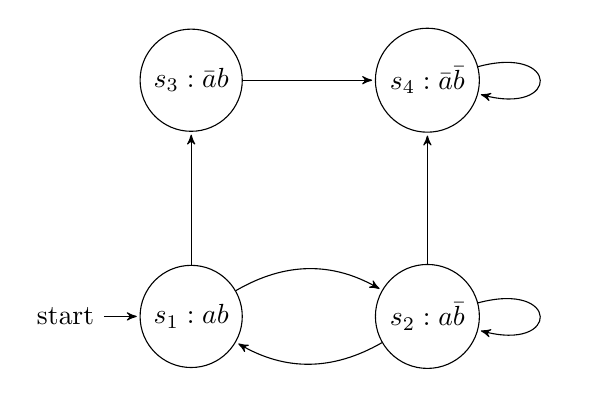
\begin{tikzpicture}[>=stealth',shorten >=1pt,auto,node distance=3cm]
  \node[state] (q3)      {$s_3: \bar a b$};
  \node[state] (q4)    [right of=q3] {$s_4: \bar a \bar b$};
  \node[initial,state] (q1)   [below of=q3]   {$s_1: a b$};
  \node[state] (q2)   [right of=q1]   {$s_2:  a \bar b$};

  \path[->] 
        (q3) edge         node {} (q4)
        (q4) edge [loop right] node {} (q4)
        (q1) edge         node {} (q3)
        (q2) edge         node {} (q4)
        (q2) edge [loop right] node {} (q2)
        (q1) edge    [bend left] node {} (q2)
        (q2) edge    [bend left] node {} (q1);
\end{tikzpicture}
\end{center}
\label{f1}
\end{figure}
  \par
  In answering the following questions, recall that all paths are
  infinite.  To indicate a path that ends with a repeated set of
  states, put parenthesis around the repeated subsequence (e.g., $(q,
  q'', q''')$.  To indicate a path in which an initial subsequence is
  followed by any possible continuing path, write ``(any)'' after
  giving the initial sequence.
  \begin{enumerate}
  \item \textbf{[8 points]} Find a path from the initial state $s_1$
    which satisfies $\Forever a$.
    \begin{answer}
    	There are multiple paths which satisfy $\Forever a$. \newline 
    	\textbf{Path}: $s_1-(s_2)$ \newline
    	\textbf{Explanation}: Starting from state $s_!$ and then repeating on state $s_2$
    	infinitely makes keeps the literal $a$ always true. Hence this path
    	satisfies $\Forever a$
    \end{answer}
    \bigskip
  \item \textbf{[8 points]} Determine whether ${\cal M}_1, s_1 \models
    \Forever a$ and explain why or why not.
    \begin{answer}
    	${\cal M}_1, s_1 \models \Forever a$ is False. \newline
    	\textbf{Explanation}: ${\cal M}_1, s_1 \models \Forever a$ means that for
    	every path in the model literal 'a' is always true. This is not the case in
    	the given model. If you consider the path $s_1s_3(s_4)$, which means
    	starting from $s_1$ then going to $s_2$ and finally looping through $s_4$,
    	we can see that $a$ is true only in first state and then remains false. 
    \end{answer}
    \bigskip
  \item \textbf{[8 points]} Find a path from the initial state $s_1$
    which satisfies $a \Until b$.
    \begin{answer}
    	There are multiple paths that satisfy $a \Until b$. \newline
    	\textbf{Path}: $s_1-s_3-(s_4)$	\newline
    	\textbf{Explanation}: The first state $s_1$ only contains literal $b$ as
    	true. Thus any path starting from state $s$ will satisfy the condition $a
    	\Until b$.
    \end{answer}
    \bigskip
  \item \textbf{[8 points]} Determine whether ${\cal M}_1, s_1 \models
    a \Until b$ and explain why or why not.
    \begin{answer}
    	${\cal M}_1, s_1 \models a \Until b$ is True and satisfies.	\newline
    	\textbf{Explanation}: For all paths starting from state $s_1$ $a \Until b$
    	is true as the first state itself contains $b$ to be true hence state $s_1$
    	will satisfy the $a \Until b$. Also according to the definition of $\Until$
    	we dont need to check further once $b$ is satisfied.
    \end{answer}
    \bigskip
  \item \textbf{[8 points]} Find a path from the initial state $s_1$
    which satisfies $\NextX a \Until \NextX (\neg a \land b)$.
    \begin{answer}
    	$\NextX a \Until \NextX (\neg a \land b)$ is satisfied in one of the many
    	paths.	\newline
    	\textbf{Path}: $s_1-s_3-(s_4)$	\newline
    	\textbf{Explanation}: In the path specified above $\NextX (\neg a \land b)$
    	is true in the state $s_1$, hence the expression is satisfied in the
    	specified above.
    \end{answer}
    \bigskip
  \item \textbf{[8 points]} Determine whether ${\cal M}_1, s_1 \models
    \NextX a \Until \NextX (\neg a \land b)$ and explain why or why not.
    \begin{answer}
    	${\cal M}_1, s_1 \models \NextX a \Until \NextX (\neg a \land b)$ is False.
    	\newline \textbf{Explanation}: Path $s_1-s_2-(s_4)$ is one of the paths in
    	the model which doesn't satisfy the expression, since $\NextX (\neg a \land
    	b)$ is never true in the path. And hence the complete expression is never
    	true. So since the expression doesn't satisfy all the possible paths, its
    	False.
    \end{answer}
    \bigskip
  \item \textbf{[8 points]} Find a path from the initial state $s_1$
    which satisfies $\NextX \neg b \land \Forever (a \lor \neg b)$.
    \begin{answer}
    	One of the multiple paths satisfy $\NextX \neg b \land \Forever (a
    	\lor \neg b)$.	\newline
    	\textbf{Path}: $s_1-s_2-(s_4)$.	\newline
    	\textbf{Explanation}: In the path above $\NextX \neg b$ is always true,
    	since from state $s_2$ onwards $\neg b$ is always true. So also the
    	expression $\Forever (a \lor b)$ is from state $s_2$ onwards and for state
    	$s_1$ the literal $a$ is true.
    \end{answer}
    \bigskip
  \item \textbf{[8 points]} Determine whether ${\cal M}_1, s_1 \models
    \NextX \neg b \land \Forever (a \lor \neg b)$ and explain why or why not.
    \begin{answer}
    	${\cal M}_1, s_1 \models \NextX \neg b \land \Forever (a \lor \neg b)$ is
    	False.	\newline.
    	\textbf{Explanation}: Consider a path $s_1-s_3-(s_4)$. In this path
    	$\NextX \neg b$ is false for the state $s_1$ and thus the entire expression
    	is false and for the state $s_3$ the second expression $(a \lor
    	\neg b)$ is false since neither $a$ nor $\neg b$ is true. Hence for this
    	path $\Forever (a \lor \neg b)$ is also false. Thus since the given
    	expression is a conjunction of both and there are states which only satisfy
    	one hence for all possible states the given expression is False.
    \end{answer}
    \bigskip
  \item \textbf{[8 points]} Find a path from the initial state $s_1$
    which satisfies $\NextX (\neg a \land b) \land \Sometime (\neg a
    \land \neg b)$.
    \begin{answer}
    	One path that satisfies the formula $\NextX (\neg a \land b) \land
    	\Sometime (\neg a \land \neg b)$.	\newline
    	\textbf{Path}: $s_1-s_3-(s_4)$	\newline
    	\textbf{Explanation}: $\NextX (\neg a \land b)$ is satisfied since $\neg a
    	\land b$ is satisfied in state $s_3$ and state $s_4$ satisfies $\neg a
    	\land \neg b)$. Hence formula $\Sometime (\neg a \land \neg b))$ is also
    	satisfied in the path.
    \end{answer}
    \bigskip
  \item \textbf{[8 points]} Determine whether ${\cal M}_1, s_1 \models
    \NextX (\neg a \land b) \land \Sometime (\neg a \land \neg b)$ and explain why or why not.
    \begin{answer}
    	${\cal M}_1, s_1 \models \NextX (\neg a \land b) \land \Sometime (\neg a
    	\land \neg b)$ is False since it is not valid for all the paths in the
    	model. \newline
    	\textbf{Explanation}: Consider a path $s_1-(s_2)$. This is one of the path
    	for which the formula is not satisfied in the model. For state $s_2$ $\neg
    	a \land b$ is not true, hence $\NextX (\neg a \land b)$ is also false for
    	state $s_1$. So first part of conjunction of the formula is false. Also to
    	add to this $\neg a \land \neg b$ is not satified in any of the state in
    	the path. Hence the formula $\Sometime (\neg a \land \neg b)$ is also
    	false. Thus for this path and the model the formula is false.
    \end{answer}
    \bigskip
  \end{enumerate}

\item \textbf{[20 points]} List all subformulas of the LTL formula
  \begin{displaymath}
    \NextX \neg p \Until (q \Until ((\Forever r \lor \NextX \Sometime
    \neg q) \implies \NextX r \WeakUntil \neg q))
  \end{displaymath}
  	\begin{answer}
    	The subformulas are as follows:- 
    	\begin{enumerate}
    	  \item $\NextX \neg p \Until (q \Until ((\Forever r \lor \NextX \Sometime
    \neg q) \implies \NextX r \WeakUntil \neg q))$
    	  \item $\NextX \neg p$
    	  \item $\neg p$
    	  \item $p$
    	  \item $q \Until ((\Forever r \lor \NextX \Sometime
    \neg q) \implies \NextX r \WeakUntil \neg q)$
    	  \item $q$
    	  \item $(\Forever r \lor \NextX \Sometime
    \neg q) \implies \NextX r \WeakUntil \neg q$
    	  \item $\Forever r \lor \NextX \Sometime
    \neg q$
    	  \item $\Forever r$
    	  \item $r$
    	  \item	$\NextX \Sometime \neg q$
    	  \item $\Sometime \neg q$
    	  \item $\neg q$
    	  \item $\NextX r \WeakUntil \neg q$
    	  \item $\NextX r$
    	\end{enumerate}
    \end{answer}
    \bigskip
\end{itemize}

\end{document}
